\section{The grammar and the seed}\label{sec:grammar}

\paragraph{The question.}
The principle says that existence is what remains when cancelling to nothing cannot complete. To ask what that forces,
the sentence has to be given a form in which something can be computed. This section gives it one: two records, two
moves and their pull-backs. It then asks the first question the form can answer, namely what the first description is
that mixes the two records and does not cancel. The answer is a theorem with four stated inputs, and the section
discloses how the answer was known before the inputs were written. All results of the program are cited by their
arcs in the repository~\cite{OriginAxiomRepo}.

\paragraph{The principle.}
We use the single wording of the record: existence is what remains when cancelling to nothing cannot complete (PF1);
that remainder is a description that cannot be exhausted (PF2); the program reads that description as mathematical
structure and asks what it forces (PF3). The three are postulated, as three faces of one commitment, and nothing in
the record derives one from another. The mathematical face of PF1 is a reading, not a derivation. For two letters $a,b$
of the once-punctured torus group it is the Fricke--Vogt invariant $\kappa=\tr[a,b]$, and cancelling to nothing
completes where $\kappa=2$. The wording is therefore that a description \emph{generically does not cancel}
($\kappa\neq 2$), never that it cannot.

\paragraph{The grammar.}
A \emph{description} is built from two integer records, $(a,b)\in\Z^2$. The grammar has five items.
\begin{itemize}
\item \emph{Records and moves} (GM1, GM2). An update acts on the pair of records. The elementary updates are the unit
  shears
  \[
    L=\begin{pmatrix}1&1\\0&1\end{pmatrix}:(a,b)\mapsto(a,a+b),\qquad
    R=\begin{pmatrix}1&0\\1&1\end{pmatrix}:(a,b)\mapsto(a+b,b),
  \]
  and a description is a word in them. Every hyperbolic class of $\SL(2,\Z)$ is, up to sign, a cyclic word in $L$ and $R$
  containing both letters (a classical fact~\cite{Series1985}; the paper's check \texttt{checks/positive\_words.py} confirms it for all $168$
  hyperbolic matrices with entries of absolute value at most $5$).
\item \emph{Aperiodicity} (GM3). The description does not repeat, so the monodromy is hyperbolic.
\item \emph{The carrier} (GM4). Words are realized as mapping classes of the once-punctured torus, whose first
  homology is $\Z^2$.
\item \emph{Reversible updates} (GM5a), with the unit shears of GM2.
\item \emph{The pull-back} (GM5b). The inverse moves $L^{-1}$ and $R^{-1}$ are legal updates.
\end{itemize}
GM5b is adopted as a reading of PF1's own cancelling, chosen on the mathematics (B1662); it is not a
derivation. In PF1's form $\kappa=\tr[a,b]$ the commutator is two letters followed by their two inverses. Among the
moves the same shape is the commutator of $LR$ and $RL$, which freely generate the commutator subgroup of $\SL(2,\Z)$,
the fundamental group of the modular once-punctured torus. This is classical; the paper's check script confirms it
(both words lie in the kernel of the abelianisation $\SL(2,\Z)\to\Z/12$, and a coset enumeration gives the subgroup they
generate index $12$).
Note that the commutator of the single letters is not of this kind: $\tr[L,R]=3$. The next two statements are the
facts the adoption rests on. Both are finite matrix computations.

\begin{proposition}[the failed cancellation and the sign]\label{prop:sign}
At the root the commutator of the two products $LR$ and $RL$ does not return to the identity. It equals $-U$ with $U$
unipotent, so its trace is $-2$: the cancellation lands on the cusp, with a sign. The sign itself is generated by the
moves and their pull-backs,
\[
  -I=(L\,R^{-1}L)^2=(L^{-1}R)^3 .
\]
\end{proposition}
\begin{proof}
Direct multiplication. $[LR,RL]=\begin{psmallmatrix}-7&6\\-6&5\end{psmallmatrix}=-U$ with $U=\begin{psmallmatrix}7&-6\\6&-5\end{psmallmatrix}$,
which has trace $2$ and is not the identity. Next, $L R^{-1}L=\begin{psmallmatrix}0&1\\-1&0\end{psmallmatrix}$ squares to $-I$, and
$L^{-1}R=\begin{psmallmatrix}0&-1\\1&1\end{psmallmatrix}$ has order six with cube $-I$. The square $(LR^{-1}L)^2=-I$ is unchanged when
$L$ and $R$ are replaced by their inverses (the mirror, B1662). The two elements fix the points $i$ and $\omega=e^{2\pi i/3}$ of the
upper half-plane, and no word in $L,R$ alone reaches them: a word in $L,R$ has non-negative entries, so $ad=1+bc\ge1$
forces $a,d\ge1$, and its trace is $2$ only when $a=d=1$, otherwise at least $3$; a finite order element has trace $0$ or
$\pm1$.
\end{proof}

The record reads the trace $-2$ through classical results and uses them only for what they say. On the character
variety of the once-punctured torus the trace of the commutator is $x^2+y^2+z^2-xyz-2$ in the traces
$(x,y,z)=(\tr a,\tr b,\tr ab)$ (Fricke's identity), and $-2$ is the value at which the commutator is parabolic: the
puncture. The modular group's action on these characters is studied in~\cite{Goldman2003}, and the classification of
the punctured-torus groups is in~\cite{Minsky1999}. We use the two references to name the setting and nothing more.

\paragraph{The direction of the moves.}
Three consequences of GM5b are readings, kept apart from the theorems.
\begin{itemize}
\item \emph{The sign is generated.} Proposition~\ref{prop:sign} shows that a full turn about a balance point negates
  both records. The place where a hand can be registered on a spin structure (B1479, B1481) is generated by the moves.
\item \emph{Positivity is the choice of side.} Step and pull-back are mirror images: conjugation by $\mathrm{diag}(1,-1)$
  sends $L$ to $L^{-1}$, $R$ to $R^{-1}$ and $\tau$ to $-\bar\tau$. The restriction to non-negative counts, which an
  earlier form of the grammar stated as a rule on states, is therefore a selection of one side of the mirror. It stays a
  chosen input. Under the pull-back the reachable updates are $\SL(2,\Z)$, and every hyperbolic class keeps a
  forward representative, so no statement about the threads changes.
\item \emph{The arrow is the escape.} A random walk with steps $L^{\pm1},R^{\pm1}$ at equal strength is transient on
  $\SL(2,\Z)$, since the group is non-amenable~\cite{Kesten1959}, and it escapes at a positive linear rate~\cite{Furstenberg1963,FurstenbergKesten1960}. These
  cover the symmetric walk; for the unequal weights of Section~\ref{sec:boundary} the rate is positive by Furstenberg's theorem, since the support
  generates $\SL(2,\Z)$, and its values are measured (B1663).
  The reading in which the pull-back only undoes the last step is recurrent at equal strength. So only the reading
  adopted here never settles at equal strength, and the arrow is the escape, a positive rate with no preferred side. We cite the two theorems and do not
  use the walk below until Section~\ref{sec:boundary}.
\end{itemize}

\paragraph{The seed.}
The first description that mixes the two records is a product of both unit moves. To see what the grammar selects, let
the increments of the shears vary: $L_a=\begin{psmallmatrix}1&a\\0&1\end{psmallmatrix}$, $R_b=\begin{psmallmatrix}1&0\\b&1\end{psmallmatrix}$ with
integers $a,b\ge1$, and set $B(a,b)=L_aR_b=\begin{psmallmatrix}1+ab&a\\b&1\end{psmallmatrix}$. The selection criterion SE1 asks that
the first homology of the mapping torus be torsion-free. Orientation (SE2) takes the orientable one of the two classes
that SE1 leaves.

\begin{theorem}[the seed, T1]\label{thm:seed}
Take GM3 (aperiodicity), GM4 (the once-punctured-torus carrier), SE1 (a torsion-free first homology) and SE2 (the
orientable choice). Then the root, the first mixed persistent sector, is the monodromy
\[
  A=LR=\begin{pmatrix}2&1\\1&1\end{pmatrix},\qquad \tr A=3,
\]
up to the order bit $LR$ against $RL$, and its mapping torus is the complement of the figure-eight knot. In
particular, on the positive grid $1\le a,b\le12$ all $144$ closures $B(a,b)$ are hyperbolic and exactly one is
torsion-free, $(a,b)=(1,1)$.
\end{theorem}
\begin{proof}[Proof (sketch; the record's uniqueness theorem, B1323, B1454)]
For $B\in\SL(2,\Z)$ one has $\det(B-I)=2-\tr B$, and the mapping torus has $H_1=\Z\oplus\mathrm{coker}(B-I)$. Hence for
$B(a,b)$: $\tr B=2+ab$, which exceeds $2$ for every $a,b\ge1$ (so all $144$ are hyperbolic), and the torsion of $H_1$
has order $ab$. It is trivial exactly when $ab=1$, that is $(a,b)=(1,1)$ and $B=LR$. On the full set of states, torsion
of order $|2-\tr|$ vanishes only for trace $3$ among the hyperbolic classes (GM3 excludes the elliptic trace $1$), and
the trace-$3$ class is that of $LR$ (the paper's check \texttt{checks/positive\_words.py} confirms it for every such matrix with entries up to $5$; the general
statement is the class-number-one fact for discriminant $5$~\cite{Buell1989}). When orientation-reversing monodromies are
admitted, the torsion has order $|\tr|$ and the torsion-free classes are those of $LR$ and of the golden matrix $LP$
(determinant $-1$, trace $\pm1$, with $(LP)^2=LR$), whose bundle is the Gieseking manifold $m000$. SE2 takes the
orientable one, $m004$, the orientation double cover of $m000$. The mapping torus of $LR$ is the figure-eight complement~\cite{Riley1975,Thurston1979}.
The words route (aperiodic $\Rightarrow$ Sturmian $\Rightarrow$ the golden matrix) and the records route are one
construction in two presentations (B1323; B1607 for the principle's tick).
\end{proof}

\noindent\emph{Scope.} The theorem is conditional on its four inputs, and each is needed: without GM3 the order-six
monodromy of trace $1$ (the trefoil complement) and the parabolic monodromies of trace $2$ also satisfy SE1; without GM4
the closed torus bundle of $LR$, which is torsion-free, remains; without SE1 every state remains; without SE2 the parent $m000$ remains. Positivity (the choice of the forward side), minimality of the trace, the unit-shear generation GM2 and
the order bit are not needed for the root. The root's uniqueness holds with and without positivity: without it the
torsion-free hyperbolic solutions are $(1,1)$ and $(-1,-1)$, in one class (B1454). The theorem selects one
\emph{thread} of the family that the grammar allows. It does not make that thread privileged, and no later result in
the paper uses it as a premise.

\begin{figure}[t]
\centering
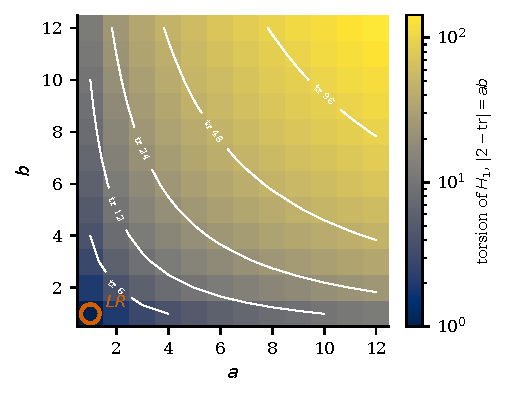
\includegraphics[width=0.62\linewidth]{figures/fig_seed}
\caption{An illustration of the identity $|H_1|=ab$, not a separate result. Torsion order $|2-\tr B(a,b)|=ab$ of $H_1$ over the $12\times12$ grid of
closures (colour, logarithmic), with contours of the trace $2+ab$. The root $LR$, $(a,b)=(1,1)$, is the only
torsion-free closure. This is an exact computation on the grid, conditional on the inputs of Theorem~\ref{thm:seed}.}
\label{fig:seed}
\end{figure}

\paragraph{Provenance.}
The root was known before the axioms were written: the figure-eight complement was named in a probe, and the grammar was
written afterwards. The genesis is therefore a conditional reconstruction of a chosen sector, not a derivation of the
figure-eight from nothing. We say so here because a reader will otherwise suspect it. No input of
Table~\ref{tab:inputs} is derived from a weaker one in the record, and none of the three further anchors proposed
within the program for the genesis is graded proved in the record (one is refuted, two are conditional).

\paragraph{The inputs.}
Table~\ref{tab:inputs} lists every input this paper uses, with its status, what it buys and what would discharge it. The
last lines of the table state the price as the record counts it.

{\footnotesize
\begin{longtable}{@{}p{3.2cm}p{2.4cm}p{3.6cm}p{6.0cm}@{}}
\caption{The inputs ledger. Status words follow the record: \emph{postulated}, \emph{chosen} (a selection),
\emph{adopted} (a ruling made on the mathematics), \emph{tagged} (a working postulate whose results carry ``given'').}\label{tab:inputs}\\
\toprule
input & status & what it buys & what would discharge it\\
\midrule
\endfirsthead
\toprule
input & status & what it buys & what would discharge it\\
\midrule
\endhead
\bottomrule
\endlastfoot
PF1--PF3, the principle & postulated & the question: what a non-cancelling description forces & none in the record\\
the grammar, GM1--GM5a & postulated (GM3 cheap; GM4's puncture conditional) & the moves, the threads, the carrier & none; GM1 is not independent of GM4\\
SE1, torsion-free first homology & postulated & the root among the states & alternatives are kept: minimal trace, minimal volume\\
SE2, orientation & chosen & the orientable root, and the sheet that carries the hand & a derived reason for orientability, or carrying both $m004$ and $m000$\\
GM5b, the pull-back acts & adopted, as a reading of PF1's cancelling & the sign $-I$ and a motion with no preferred side at equal strength; not needed for the root & not a derivation\\
positivity, as the side & chosen (a selection) & one side of the mirror: forward words & a reason for the side; what CP violation would read\\
the triplet postulate & tagged & left-handed matter in the triplet $T$; the mass tensor & a derivation of which fields carry $T$ (the dictionary), or an obstruction; an index for the count does not pay it\\
one cusp unit & tagged & the index $\pm3$ (Section~\ref{sec:three}) & an end mechanism at the cusp\\
the extreme boundary domain & chosen & $|\Lambda_+|\in\{0,6\}$, so $\pm3$ rather than $\pm1$ (Section~\ref{sec:three}) & a rule that selects the domain\\
$M_{1,2}$ as the weave's surface & a reading, verified in part & the setting of the index and of the zero modes & coherence of the lifts (a gate still open)\\
the vacuum-grading rule (demand D1, Section~\ref{sec:boundary}) & a ruling of the program & how a symmetry broken by a vacuum is graded & none\\
the end condition at the puncture (equal canonical amplitudes) and the choice of canonical horocycle & chosen (the horocycle a discrete choice; the radius of order one, Census law~\ref{cl:cusp}) & the norm of the boundary class, the lepton sector's null vector, the symmetric point's law, the census N5 and the first generation's lift (Sections~\ref{sec:couplings}, \ref{sec:three}) & an end mechanism at the puncture, or a reason for one horocycle\\
the modulus $\tau=\omega$ and the eighteen flat lines & chosen (a selection, Section~\ref{sec:selection}) & the lepton sector's null vector, the symmetric point and the one-Higgs census N5 (Sections~\ref{sec:couplings}, \ref{sec:boundary}) & a rule that selects the modulus and the lines\\
equal framed data & chosen & the twisted half bound & a reason that the sectors' framed data are equal\\
the index as the generation count & identification & reads the index $\pm3$ of Section~\ref{sec:three} as three generations & an index theorem on a physical spacetime\\
the read-out and the hypercharge dictionary & identifications & singular values as masses, flat-line twists as hypercharges and the Higgs line as the electroweak Higgs, with $6Y$ the minimal integral normalisation, itself a choice (Sections~\ref{sec:couplings}, \ref{sec:boundary}) & a derivation of the dictionary\\
the fibre frame (the Higgs a section on the fibre, at one $\tau$) & chosen (see Verdict~\ref{bd:tribunal}) & the couplings of Section~\ref{sec:couplings} & a frame shown to meet the demands\\
the Higgs's type and locus (a point or density Higgs, at the puncture) & stated & the covariance theorem and the rank of a point coupling (Section~\ref{sec:couplings}) & a Higgs of another type, or a derived locus\\
zero Wilson line on the fibre & stated (a restriction of the frame) & the isotropy theorem and its null vector (Section~\ref{sec:couplings}) & a derivation of the connection, or the theorem for a non-zero line\\
the hand and the $\eta$ twist & chosen conventions, not derived & $\rho$ as the theta multiplier (Section~\ref{sec:modular}) & a derived hand; a reason for the twist\\
the modular-flavour ansatz (holomorphic couplings, a minimal K\"ahler term, one copy of $T$ per field, one Higgs per sector) & stated where used, not adopted & the ruled-branch bound of Theorem~\ref{bd:reducesnone}; the half floor and the determinant laws of Section~\ref{sec:anomaly} (with real coefficients where the strong angle is read) & none\\
the moves as a symmetry of the fermions, with weights, and $\tau$ a field & stated where used & the anomaly of the moves and the strong angle's transformation (Section~\ref{sec:anomaly}) & a derivation that the moves act on the fermions as a symmetry\\
the Dedekind counterterm $\theta(\tau)=\theta_0+6K\arg\eta(\tau)$ & stated where used (an input with a field: $\mathrm{Re}\,\tau$ coupled to the gluons' $G\tilde G$) & a strong angle invariant under the moves (Proposition~\ref{prop:strong}) & a mechanism that supplies it, or weights with no anomaly\\
the index formula $\dim\Lambda_+-3$ & taken as stated (B1606) & the index of Section~\ref{sec:three} & an independent derivation\\
\midrule
\multicolumn{4}{@{}p{15.4cm}@{}}{\textbf{Price.} The rows above are this paper's inputs. For comparison, the
record's identification ledger, which prices the program's whole chain to the Standard Model including frames this paper
does not use, counts four axioms and nine irreducible identifications; this paper uses three of the nine (the triplet
postulate, the index as the generation count, and the read-out with its dictionary). The modulus $\tau$ and the
choice of canonical horocycle are not rows of that ledger. Against the Standard Model's nineteen values the paper derives
none.}\\
\end{longtable}}

\reading{The arena. SE1 has two solutions: trace $3$, the root, and trace $1$, the order-six move $L^{-1}R$ whose mapping
torus is the trefoil complement. Under the pull-back the second is reached by the moves (it fixes $\omega$), and GM3
keeps it from being a thread. We read the root as the motion and the trace-$1$ solution as the arena the motion
moves in: $\SL(2,\R)/\SL(2,\Z)$ is the complement of the trefoil~\cite{Milnor1971}, and the closed orbits of its
geodesic flow are the threads~\cite{Ghys2007}. The classical facts are cited, and nothing in the paper is derived from
this reading.}
